\documentclass[11pt, landscape]{article}
\usepackage[utf8]{inputenc}
\usepackage[T1]{fontenc}
\usepackage[german=swiss]{csquotes}
\usepackage{multicol}
\usepackage{multirow}
\usepackage[ngerman]{babel}
\usepackage[a4paper, landscape, margin=15mm]{geometry}
\usepackage[colorlinks=true, citecolor=blue, linkcolor=blue, urlcolor=blue]{hyperref}
\usepackage{graphicx}
\usepackage{enumitem}
\usepackage{tikz}
\usepackage{xcolor}
\usepackage[backend=biber, style=authortitle, bibencoding=auto]{biblatex}
\usepackage[medium, compact, explicit]{titlesec}
\usepackage{xurl}
\usepackage{fancyhdr}
\usepackage{tabularx}
\usepackage{booktabs}
\usepackage{makecell}
\usepackage{afterpage}
\usepackage{emptypage}
\usepackage{layouts}

% sans-serif urls
\urlstyle{same}

% color box command
\newcommand\cbox[2][black]{\textcolor{#1}{\rule{#2}{#2}}}

% bibliography setup
\addbibresource{./bibliography.bib}
\setlength{\bibhang}{0pt}
\setlength{\bibitemsep}{8pt}
\DeclareFieldFormat{url}{\url{#1}}

% above 30°
\definecolor{above30}{HTML}{f2e50a}
\definecolor{above35}{HTML}{f46f24}
\definecolor{above40}{HTML}{de055b}
\definecolor{tooSteep}{HTML}{c889bb}

% set sans serife font as default
\renewcommand{\familydefault}{\sfdefault}

% remove section numbers
\titleformat{name=\section}{\normalfont\Large\bfseries}{}{0pt}{#1}
\titleformat{name=\subsection}[block]{\normalfont\normalsize\itshape}{\hspace{6mm}}{\columnwidth}{\vspace{-26pt}\smash{\parbox[l][9pt]{35mm}{#1}}}{}

\graphicspath{ {./media} }

% adjust paragraph margins
\setlength{\parindent}{0pt}
\setlength{\parskip}{8pt}

% adjust list styles
\setlist[enumerate]{nosep, leftmargin=12pt, labelsep=3pt}
\setlist[itemize]{nosep, leftmargin=10pt, labelsep=3pt}

% disable head rule
\renewcommand{\headrulewidth}{0pt}

% qr code figure
\newcommand\qrcode[3]{
  \begin{tabularx}{\linewidth}{lcl}
    \makecell[l]{\includegraphics[width=0.24\linewidth]{#1}} & \makecell[c]{\hspace{8pt}{ }} & \makecell[X]{#3\\\footnotesize{\href{https://#2}{#2}}}
  \end{tabularx}
}

\setlength{\tabcolsep}{0pt}

% meta data
\title{Merkblatt Skitouren}
\author{SAC Aarau}
\date{\today}

\begin{document}
  \pagestyle{fancy}
  
  \fancyhead{}

  \fancyfoot[L]{\footnotesize{Merkblatt Skitouren}}
  \fancyfoot[C]{\footnotesize\thepage}
  \fancyfoot[R]{\footnotesize{Publiziert am \today}}

  \nocite{*}
  \afterpage{
    \newgeometry{a4paper, landscape, margin=15mm, right=61.842515mm}

    \setlength{\columnsep}{46.842515mm}

    \begin{multicols*}{2}[
      \parbox{267mm}{
        \vspace{-15mm}
        \maketitle
        \vspace{-5mm}
        \thispagestyle{fancy}
      }
    ]
      \section{Rund um das LVS}

\subsection{Die Antennen}

Alle modernen Geräte verfügen über 3 Antennen.

Es sendet jeweils nur eine Antenne.

Im Suchmodus empfangen alle Antennen.

\begin{center}
  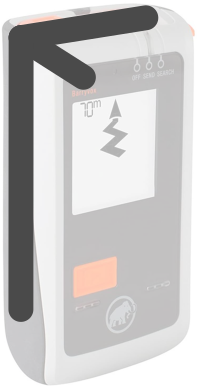
\includegraphics[width=0.5\linewidth]{antennas.svg.pdf}
\end{center}

Die Antennen sind empfindlich gegen Erschütterungen, es ist also behutsam mit dem LVS umzugehen um den Bruch einer oder mehrerer Antennen zu vermeiden.

\newcolumn

\subsection{Was sind Störquellen und Interferenzen?}

Elektronische Geräte und metallische Gegenstände stören das LVS bei der Arbeit, darum gilt:

\begin{itemize}
  \item{Im Sendemodus mindestens 20 cm Abstand}
  \item{Im Suchmodus mindestens 50 cm Abstand}
  \item{Während einer Verschüttetensuche mindestens 10 m Abstand zu Mobiltelefone und Funkgeräte im aktiven Betrieb (Funken bzw. Telefonieren)}
\end{itemize}

\textit{Die modernen LVS weisen im Suchmodus auch akustisch und/oder visuell auf eine vorhandene Störquelle hin.}

\subsection{Wie funktioniert die Suche mit dem LVS?}

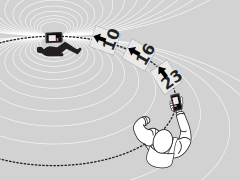
\includegraphics[width=\linewidth]{lvs-search.svg.pdf}

Das Gerät leitet die Suche entlang der Feldlinien: \textit{Es ist also völlig normal bei der Suche eine Kurve zu beschreiten.}

\newcolumn

Die effektive Reichweite eines LVS ist Geräteabhängig. In der Praxis hat sich eine Suchstreifenbreite von ca. 40 m bewährt. Also vom Gerät ausgehend 20 m in jede Richtung.

Die Distanzangabe auf dem Gerät entspricht in etwa der Kurvenlänge auf der Feldlinie.

\subsection{Der Suchvorgang}

Um die Suchrichtung festzustellen muss das Gerät in Bewegung sein: \textit{Ich kann also nicht an einem Ort stehen bleiben um die Suchrichtung zu bestimmen.}

Die Suche mit dem LVS unterteilt sich in 4 Phasen:

\begin{enumerate}
  \item{
    \textbf{Signalsuche} -- solange kein Signal empfangen
    \begin{itemize}
      \item{Suche nach optischen Hinweisen}
      \item{Suche nach akustischen Hinweisen}
      \item{Suche nach erstem Signal mit dem LVS}
    \end{itemize}
  }
  \item{
    \textbf{Grobsuche} -- bis auf 3 m 
    \begin{itemize}
      \item{Der Richtungsangabe auf dem LVS folgen}
      \item{Ruckartige Bewegungen vermeiden}
      \item{Ab 10 m Schritttempo verlangsamen}
    \end{itemize}
  }
  \item{
    \textbf{Feinsuche} -- bis Minimaldistanz
    \begin{itemize}
      \item{Suche etwa auf Kniehöhe}
      \item{LVS nicht mehr neu ausrichten}
      \item{Suche nach Minimaldistanz}
    \end{itemize}
  }
  \item{
    \textbf{Punktsuche} -- bis Treffer mit der Sonde
    \begin{itemize}
      \item{Sondieren, ausgehend von Minimaldistanz}
      \item{Bei Treffer Sonde stecken lassen}
      \item{Umgehend mit der Bergung beginnen}
    \end{itemize}
  }
\end{enumerate}

Es gilt schnellstmöglich Kopf und Brustkorb des Lawinenopfers freizulegen.
Ohne Lebenszeichen sofort mit der Reanimation beginnen.

Ist das Lawinenopfer bei vollem Bewusstsein, soll das Wiederaufwärmen durch aktive Bewegung und warme Getränke erfolgen.

\newcolumn

Bei Bewusstseinstrübung oder Ohnmacht sollten weitere Bewegungen allerdings vermieden werden: Stattdessen vor weiterem Auskühlen schützen und nach Möglichkeit warme Getränke verabreichen.

\begin{center}
  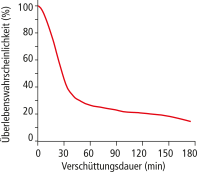
\includegraphics[width=0.9\linewidth]{ueberlebenswahrscheinlichkeit.svg.pdf}
\end{center}

\textbf{Bei einem Lawinenunfall sind die ersten 15 Minuten entscheidend, danach sinkt die Überlebenschance deutlich.}

\newcolumn

\subsection{Wie wird das LVS korrekt getragen?}

Es wird empfohlen das LVS mit dem dazugehörigen Gurtsystem zu tragen.
Dabei sollte das LVS immer von mindestens einer Schicht Kleidung bedeckt sein.

\begin{center}
  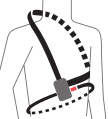
\includegraphics[width=0.48\linewidth]{lvs-harness.svg.pdf}
  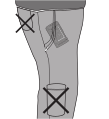
\includegraphics[width=0.48\linewidth]{lvs-pocket.svg.pdf}
\end{center}

Alternativ kann das LVS auch in einer Hosentasche mitgeführt werden.
Für die Hosentasche gilt dabei:

\begin{itemize}
  \item{Sie muss über einen Reissverschluss verfügen.}
  \item{Sie darf nicht auf die Hose aufgenäht sein.}
  \item{Gesässtaschen sind nicht geeignet.}
\end{itemize}

Das LVS sollte am Anfang der Saison mit frischen Batterien bestückt werden.
Damit die Batterien nicht auslaufen und das Gerät beschädigen können sollten diese am Ende der Saison herausgenommen werden.
\textbf{Keine wiederaufladbaren Batterien verwenden.}

Die genaue Laufzeit ist abhängig vom Gerät, beträgt im Sendemodus aber in etwa 200 Stunden.
Im Suchmodus hingegen nur 1 Stunde.

\textbf{Das LVS muss während der gesamten Tour im Sendemodus eingeschaltet sein.}
Ausschalten auf dem Gipfel oder während einer Pause zum Batterien sparen ist nicht notwendig.

\newcolumn

      \section{Kleine Lawinenkunde}

Das Lawinenbulletin ist eine \textbf{Prognose der Lawinengefahr} für eine geografische Region und \textbf{nicht für den Einzelhang}.

Die Hauptausgabe des Lawinenbulletin erscheint um 17 Uhr auf der Website des SLF \href{https://www.slf.ch}{www.slf.ch} und in der App \enquote{White Risk}.
Je nach Situation erscheint morgens um 8 Uhr eine weitere Ausgabe.

Die Lawinengefahr wird mit der \textit{Gefahrenstufe} inklusive \textit{Geltungsbereich} und den typischen \textit{Lawinenproblemen} angegeben.

\begin{center}
  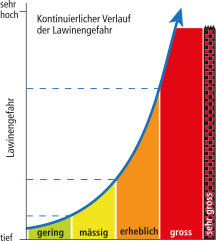
\includegraphics[width=0.82\linewidth]{bulletin.svg.pdf}
\end{center}

Die \textbf{Gefahrenstufen} gibt uns eine erste Einschätzung über die prognostizierte Lawinensituation in der Region.

\newcolumn

Folgende Gefahrenstufen sind definiert:

\begin{enumerate}
  \item{
    \textbf{Gering} -- günstige Situation
    \begin{itemize}
      \item{Es sind keine Alarmzeichen feststellbar.}
      \item{Extrem steile Hänge einzeln befahren.}
      \item{Absturzgefahr beachten.}
      \item{Für etwa 20\% des Winters prognostiziert.}
      \item{Rund 5\% aller Todesopfer.}
    \end{itemize}
  }
  \item{
    \textbf{Mässig} -- mehrheitlich günstige Situation
    \begin{itemize}
      \item{Vereinzelt sind Alarmzeichen feststellbar.}
      \item{Vorsichtige Routenwahl, vor allem im angegebenen Geltungsbereich des Bulletin.}
      \item{Für etwa 50\% des Winters prognostiziert.}
      \item{Rund 30\% aller Todesopfer.}
    \end{itemize}
  }
  \item{
    \textbf{Erheblich} -- kritische Situation
    \begin{itemize}
      \item{Wummgeräusche und Risse sind typisch.}
      \item{Defensive Routenwahl ist empfohlen.}
      \item{Sehr steile Hänge meiden.}
      \item{Unerfahrenen wird empfohlen zu verzichten.}
      \item{Für etwa 30\% des Winters prognostiziert.}
      \item{Rund 50\% aller Todesopfer.}
    \end{itemize}
  }
  \item{
    \textbf{Gross} -- sehr kritische Situation
    \begin{itemize}
      \item{Spontane Lawinen sind wahrscheinlich.}
      \item{Auf mässig steiles Gelände beschränken.}
      \item{Unerfahrenen wird empfohlen zu verzichten.}
      \item{Für wenige Tage im Winter prognostiziert.}
      \item{Rund 10\% aller Todesopfer.}
    \end{itemize}
  }
  \item{
    \textbf{Sehr Gross} -- ausserordentliche Situation
    \begin{itemize}
      \item{Sehr grosse Lawinen sind zu erwarten.}
      \item{Strassen und Dörfer in Tallage sind gefährdet.}
      \item{Verzicht auf Schneesport abseits geöffneter Abfahrten und Routen wird empfohlen.}
      \item{Wird sehr selten prognostiziert.}
      \item{Rund 1\% aller Todesopfer.}
    \end{itemize}
  }
\end{enumerate}

\newcolumn

Bei einem trockenen Lawinenproblem wird zudem eine Zwischenstufe mittels Minus ($-$) Gleich ($=$) oder Plus ($+$) angegeben.

\textit{Das bedeutet nicht, dass wir bei einem 3$-$ mehr riskieren dürfen. Für die Entscheidung ausschlaggebend ist immer die Hauptstufe.}

\begin{center}
  
\includegraphics[width=0.8\linewidth]{gefahrenplot.svg.pdf}
\end{center}

Der \textbf{Geltungsbereich} beschreibt \textit{wo} -- und gegebenenfalls \textit{wann} -- die Gefahrenstufe gilt.
Dies umfasst folgende Informationen:

\begin{itemize}
  \item{\textbf{Höhenlage} -- In welcher Höhe gilt die Gefahrenstufe. Hier wird entweder eine minimale oder maximale Höhe angegeben.}
  \item{\textbf{Exposition} -- Für welche Hanglage gilt die Gefahrenstufe. Hier wird ein Abschnitt auf der Kompassrose angegeben.}
  \item{\textbf{Tageszeit} -- Ab welcher Tageszeit gilt die Gefahrenstufe. Wird nur genannt, wenn sich die Gefahrenstufe im Tagesgang markant ändert.}
\end{itemize}

Das typische \textbf{Lawinenproblemen} schliesslich beschreibt die Schneeschicht, von der bei der genannten Gefahrenstufe und im Geltungsbereich die Hauptgefahr ausgeht.
Dies umfasst folgende Situationen:

\begin{itemize}
  \item{
    \textbf{Altschnee} -- bei einer Schwachschicht
    \begin{itemize}
      \item{Physikalische Prozesse auf und in der Schneedecke verändern deren Struktur und Stabilität.}
      \item{Wummgeräusche sind ein Alarmzeichen}
      \item{Lawinen können auch bei mässiger Lawinengefahr gefährlich gross werden!}
      \item{Gefahr droht vor allem dort, wo die Schwachschicht nahe an der Oberfläche ist.}
    \end{itemize}
  }
  \item{
    \textbf{Neuschnee} -- bei frisch gefallenem Schnee
    \begin{itemize}
      \item{Kann als Schneebrettlawine abgleiten}
      \item{Frische Schneebrettlawinen sind ein Hinweis}
      \item{Verbreitung der Gefahrenstellen meist flächig}
      \item{In der Höhe oft kritischer}
    \end{itemize}
  }
  \item{
    \textbf{Triebschnee} -- von Wind verfrachtetem Schnee
    \begin{itemize}
      \item{Frischer Triebschnee ist oft sehr auslösefreudig}
      \item{Kann als Schneebrettlawine abgleiten}
      \item{Rissbildung und frische Schneebrettlawinen können auf die Gefahr hinweisen}
      \item{Sastrugi, Wechten und Dünen sind Anzeichen dafür, dass der Wind gewütet hat}
      \item{Triebschnee sammelt sich im Windschatten.}
    \end{itemize}
  }
  \item{
    \textbf{Nassschnee} -- bei Wärme und/oder Regen
    \begin{itemize}
      \item{Nasse Lawinen können spontan und auch bei einer Hangneigung unter 30° abgehen.}
      \item{Im Frühling wird oft im Tagesgang ein Nassschnee Problem prognostiziert.}
      \item{Ein früher Start und eine frühzeitige Rückkehr ist empfohlen.}
      \item{Bei einer Warmwetterphase oder ungenügender Abstrahlung Abkühlung abwarten.}
    \end{itemize}
  }
  \item{
    \textbf{Gleitschnee} -- bei Rissen (sog. Fischmäuler)
    \begin{itemize}
      \item{Oft auf glattem Untergrund und stark besonnten Hängen.}
      \item{Die Gefährdung durch Gleitschnee ist meist von untergeordneter Bedeutung.}
      \item{Gleitschneelawinen können \textit{nicht} durch eine Person ausgelöst werden.}
      \item{Bereiche unterhalb von Gleitschneerissen sollten gemieden oder zügig passiert werden.}
    \end{itemize}
  }
\end{itemize}

\newcolumn

Für trockene Lawinen gibt es ein nützliches Hilfsmittel: Die grafische Reduktionsmethode.
Die grafische Reduktionsmethode bietet eine grobe Beurteilung der Lawinenauslösewahrscheinlichkeit.

\begin{center}
  \includegraphics[width=0.95\linewidth]{risikomatrix.svg.pdf}
\end{center}

\newcolumn
      \section{Tourenplanung}

\subsection{Tourenplanung nach dem 3x3 Raster}

Die Tourenplanung ist bis zum Tourenende ein ständiger Prozess, wobei die möglichen Entscheidungen immer weniger werden.

Wir planen eine Tour nach dem 3x3 Raster.

Dabei betrachten wir die drei \textit{Faktoren}:

\begin{itemize}
  \item{
    \textbf{Verhältnisse} -- Wetter, Bulletin, Tourenberichte
    \begin{itemize}
      \item{\href{https://www.meteoschweiz.admin.ch/}{www.meteoschweiz.admin.ch}, MeteoSwiss App}
      \item{\href{https://www.slf.ch/}{www.slf.ch}, White Risk App}
      \item{\href{https://www.gipfelbuch.ch/}{www.gipfelbuch.ch}, Hüttenwart, Bergführerbüro}
    \end{itemize}
  }
  \item{\textbf{Gelände} -- Route, Karte, Führerliteratur
    \begin{itemize}
      \item{\href{https://s.geo.admin.ch/y34y7btkqsvz}{www.map.geo.admin.ch}, White Risk App}
      \item{\href{https://www.skitourenguru.com//}{www.skitourenguru.com}}
      \item{\href{https://www.sac-cas.ch/de/huetten-und-touren/sac-tourenportal/}{www.sac-cas.ch}, SAC-CAS App}
    \end{itemize}
  }
  \item{\textbf{Mensch} -- Gruppe, Technik, Kondition, Material}
\end{itemize}

Zu unterschiedlichen \textit{Zeitpunkten}:

\begin{itemize}
  \item{\textbf{Planung} -- zu Hause, in der Hütte}
  \item{\textbf{Vor Ort} -- Ausgangspunkt, Unterwegs}
  \item{\textbf{Einzelhang} -- vor jedem Hang, Schlüsselstelle}
\end{itemize}

Jeder Faktor muss zu jedem Zeitpunkt stimmig sein.
Sobald ein Faktor nicht mehr passt entsteht ein \textit{Riskio}.
Dieses Risiko muss dann mit einer geeigneten Massnahme vermindert werden.
\textbf{Bei zwei und mehr Risikofaktoren sollten wir verzichten oder die Tour abbrechen.}

\textit{Eine gefährliche Situation entsteht meist nicht zufällig und aus dem nichts, sondern ist das Resultat einer Verkettung unvorteilhafter Entscheidungen.}

\newcolumn

\subsection{Wie finde ich eine geeignete Tour?}

Die Auswahl einer geeigneten Tour ist nicht immer ganz einfach.
An erster Stelle steht natürlich immer die Sicherheit.
Für unsere Entscheidung können wir unter anderem folgende Kriterien einfliessen lassen:

\begin{itemize}
  \item{Welche Lawinensituation herrscht in dem Gebiet?}
  \item{
    Welches Wetter herrscht(e) in dem Gebiet?
    \begin{itemize}
      \item{Windstärke? Windrichtung?}
      \item{Sonnenschein oder Wolkendecke?}
      \item{Wie viel Niederschlag ist gefallen?}
      \item{Kalte oder eher warme Temperaturen?}
    \end{itemize}
  }
  \item{
    Wie ist die Schneedecke aufgebaut?
    \begin{itemize}
      \item{Liegt überhaupt genug Schnee?}
      \item{Pulverschnee oder Bruchharsch?}
    \end{itemize}
  }
  \item{Mit welcher Schwierigkeit ist die Tour bewertet?}
  \item{Höhenmeter, Distanz und Zeitbedarf?}
  \item{Ist die Tour stark oder schwach frequentiert?}
  \item{Erreichbarkeit mit dem ÖV oder Parkplätze?}
\end{itemize}

\subsection{Wo finde ich den besten Pulverschnee?}

Oft suchen wir auf Skitouren den besten Pulverschnee.
Um die Schneelage einzuschätzen eignet sich die \textit{Schneehöhenkarte} des SLF (wird jeweils um 7 Uhr aktualisiert).
Um die Neuschnee reichen Gebiete zu finden kann die \textit{Neuschneekarte} konsultiert werden.
Auch Webcams aus dem Gebiet können hilfreich sein.
Ausserdem können folgende Faustregeln aus der Meteorologie helfen:

\begin{itemize}
  \item{Pro 100 hm nimmt die Temperatur etwa 1 °C ab.}
  \item{Pro 1 mm Niederschlag fällt rund 1 cm Schnee.}
  \item{Schnee fällt ab der Nullgradgrenze.}
\end{itemize}

\textit{So können wir -- ausgehend von einer beliebigen Wetterstation im Gebiet -- die Chance auf Neuschnee in etwa abschätzen.}

\newcolumn

\subsection{Welche Touren eignen sich für Neulinge?}

Auch als absolute Skitouren Neulinge gibt es einige Touren, welche sich ohne grosse Erfahrung sicher begehen lassen:

\begin{itemize}
  \item{Laucherenstöckli, bei Ibergeregg}
  \item{Wildspitz, oberhalb Steinerberg}
  \item{Rägeflüeli, im Eigental beim Pilatus}
  \item{Rossstock, in der Lidernen}
  \item{Firsthöreli und Mattner First, im Bisistal}
  \item{Rickhubel, am Glaubenbergpass}
  \item{Mariannenhubel, im Diemtigtal}
  \item{Meniggrat, im Diemtigtal}
\end{itemize}

\subsection{Empfehlungen zur Sicherheit}

Der Sicherheit wegen noch ein paar Empfehlungen:

\begin{itemize}
  \item{Nur bei Lawinenstufe Mässig oder Gering gehen.}
  \item{Nur bei schönem Wetter und guter Sicht unterwegs sein -- der Helikopter fliegt bei Nebel nicht.}
  \item{Nicht alleine auf Skitour gehen.}
  \item{Bei Neuschnee etwas später aufbrechen, so ist ziemlich sicher bereits eine Spur vorhanden.}
  \item{Entlang vorhandener Spuren abfahren.}
  \item{Nichts überstürzen und genug Zeit einplanen.}
  \item{Im Zweifelsfall abbrechen.}
\end{itemize}

Zum Training eignet sich auch Aufstieg und Abfahrt in einem Skigebiet.
\textit{Dies wird in einigen Skigebieten allerdings nicht gerne gesehen.}

      \section{Orientierung und Karten lesen}

Die Orientierung im winterlichen Gebirge hat seine ganz eigenen Herausforderungen.
Wir können nicht einfach einem Pfad, Wegspuren, Steinmännern oder Markierungen folgen.
Sondern müssen uns -- falls keine Spur vorhanden ist -- den Weg selbst suchen.
Auch eine vorhandene Spur ist mit Vorsicht zu geniessen und nicht immer hilfreich.

Einige Hilfsmittel können uns hier unterstützen:

\begin{itemize}
  \item{Höhenmesser, Kompass, Papierkarten}
  \item{GPS, Smartphone}
  \item{\href{https://s.geo.admin.ch/y34y7btkqsvz}{www.map.geo.admin.ch}}
  \item{\href{https://www.skitourenguru.com//}{www.skitourenguru.com}}
  \item{White Risk App (kostenpflichtig)}
  \item{swisstopo App}
\end{itemize}

\textit{Smartphone und GPS sind nützlich -- wir sollten uns aber niemals ausschliesslich darauf verlassen.}

Eine Karte in Papierform kann nicht kaputt gehen, hat keine Batterie oder Akku und ist somit ein sehr robustes Navigationsmittel.

\textit{Vorsicht bei selbst gedruckten Karten, ihr Massstab kann täuschen.}

Im Winter besonders hilfreich sind die sogenannten Hangneigungsklassen.
Hier ist die Hangneigung ab 30° in 5° Schritten farblich kodiert:

\cbox[white]{10pt} keine Färbung, mässig steil, unter 30°\\
\cbox[above30]{10pt} gelb, steil, über 30°\\
\cbox[above35]{10pt} orange, sehr steil, über 35°\\
\cbox[above40]{10pt} rot, extrem steil, über 40°\\
\cbox[tooSteep]{10pt} violett, über 45°

Im Gelände können wir folgende Faustregeln verwenden um die Hangneigung abzuschätzen:

\begin{itemize}
  \item{Unter 30° können wir Kurven laufen.}
  \item{Ab 30° müssen wir Spitzkehren machen.}
  \item{Fels durchsetztes Gelände ist oft über 40° steil.}
\end{itemize}

\newcolumn

Schlechte Sicht durch diffuse Verhältnisse, Nebel oder Schneefall können die Orientierung im Gelände erheblich erschweren.
Im Zweifelsfall können wir der vorhandenen Spur entlang zurückfinden.
Vorsicht aber bei starkem Wind oder Schneefall, dieser kann uns in kurzer Zeit die Spur zunichte machen.

Nicht ausser Acht lassen sollten wir Wildruhezonen und Schutzgebiete.
Wir unterscheiden zwei Kategorien:

\begin{itemize}
  \item{\textbf{Rechtsverbindlich} -- hier droht ein Bussgeld}
  \item{\textbf{Empfohlen} -- nach Möglichkeiten meiden}
\end{itemize}

In der Regel finden sich am Ausgangspunkt und manchmal entlang der Route im Gelände Hinweistafeln.
Offizielle  Routen und Korridore sind meist auch im Winter mit Wegweiser gekennzeichnet.
\href{https://www.respektiere-deine-grenzen.ch/}{www.respektiere-deine-grenzen.ch}

      \section{Ein paar Worte zur Ausrüstung}

Um die geeignete Bekleidung für eine Skitour zu finden können wir uns grundsätzlich an den Sommertouren orientieren und eine Schicht hinzufügen.

Wir kleiden uns nach dem Zwiebelprinzip: Viele dünne Schichten sind besser als wenige Dicke.

Eine gute \textit{Tourenbekleidung} schützt vor Wind, Nässe und Kälte -- transportiert aber auch den Schweiss nach aussen.

\begin{itemize}
  \item{Thermo Unterwäsche}
  \item{Skisocken}
  \item{Tourenhosen -- bei nasser Witterung wasserdicht}
  \item{Fleecjacke oder Pullover -- bevorzugt mit Kapuze}
  \item{Hardshelljacke -- Wind- uns Wasserdicht}
  \item{Daunenjacke}
  \item{Buff, Halstuch oder Sturmhaube}
  \item{Kappe -- bevorzugt winddicht}
  \item{Sonnenhut -- bei schönem Wetter}
  \item{dünne und robuste Handschuhe}
  \item{dicke und warme Handschuhe}
  \item{Sonnenbrille -- Schutzklasse 4}
  \item{Tourenskischuhe -- mit Gummisohle}
\end{itemize}

\textit{Die Hosen sollten auch im Aufstiegsmodus über die Skischuhe reichen und trotzdem nicht zu locker sitzen.}

Leichte und aufstiegsorientierte Skischuhe sind zwar angenehm zu tragen, machen sich aber durch ihre fehlende Stabilität meist negativ auf der Abfahrt bemerkbar -- insbesondere bei schwierigen Schneeverhältnissen.

\textit{Der etwas schwerere Schuh mit 3 oder 4 Schnallen ist also dem leichten Modell mit Klettverschluss und 1 oder 2 Schnallen vorzuziehen.}

Ausserdem benötigen wir eine \textit{Tourenausrüstung}:

\begin{itemize}
  \item{Rucksack -- etwa 30 l für eine Wochenendtour}
  \item{Teleskopstöcke -- mit grossen Tellern}
  \item{Tourenski -- mit eingestellter Bindung}
  \item{Steigfelle -- passend zum Ski}
  \item{Harscheisen -- passend zu Ski und Bindung}
  \item{Stirnlampe -- besonders im Hochwinter}
  \item{Sonnencreme -- vor allem im Frühling}
\end{itemize}

\textit{Der Rucksack sollte über eine Befestigungsmöglichkeit für Ski, Stöcke und Pickel verfügen.}

\newcolumn

\textit{Schneesportgeräte für die Piste eignen sich durch ihre Geometrie und Gewicht nur äusserst bedingt für den Toureneinsatz.}

Kurze Ski erleichtern die Spitzkehre im Aufstieg und sind wendiger auf der Abfahrt, allerdings auch etwas nervöser.
Verlangen also nach mehr Kontrolle. Die Skilänge ist abhängig von der Körpergrösse und sollte ab Boden etwa zwischen Kinn und Stirn liegen.

Ein klassischer Tourenski ist unterhalb der Bindung etwa 88 mm breit.
Wer mehr auf Abfahrt setzt greift zum etwas breiteren Ski mit 95 mm oder breiter.

Tourenski unterscheiden sich vom Pistenski neben dem Gewicht vor allem durch die früher auf biegende Skispitze.
Dadurch erhält der Ski im Tiefschnee mehr Auftrieb.
Gleichzeitig verringert sich bei harten Bedingungen und auf der Piste aber die Kontaktfläche zwischen Schneeoberfläche und Ski.
Womit der Ski während der Fahrt nervöser und schwerer zu kontrollieren wird.

Bei der Bindung hat sich das Pin System durchgesetzt.
Diese zeichnet sich durch geringeres Gewicht und besseren Drehpunkt im Aufstieg aus.
Tourenskischuh und Bindung sind in der Regel frei kombinierbar.
Beim Kauf eines Occasion Ski sollte allerdings die Sohlenlänge beachtet werden.

Ohne Rennambitionen sollte darauf geachtet werden, dass bei der Bindung der sogenannte Z-Wert eingestellt werden kann.
Der persönliche Z-Wert sollte sich ausserdem nicht gerade am Anfang oder Ende des einstellbaren Bereichs befinden.
Da wir Abseits eher langsamer unterwegs sind empfiehlt es sich den Z-Wert etwas tiefer als beim Pistenski zu wählen.

Neben geeigneter Bekleidung und Tourenausrüstung benötigen wir eine \textit{Notfallausrüstung}:

\begin{itemize}
  \item{LVS -- mit 3 Antennen und genug Batterieladung}
  \item{Lawinensonde -- aus Alu oder Carbon}
  \item{Lawinenschaufel -- mit einem Metallblatt}
  \item{Lawinenairbag -- kann Leben retten}
  \item{Helm -- ist sehr empfohlen}
\end{itemize}

\textit{Eine gute Schaufel kann im Notfall zwischen Leben und Tod entscheiden. Wir tragen dieses wichtige Ausrüstungsstück nicht für uns mit -- sondern für alle anderen.}

Im weiteren benötigen wir innerhalb der Gruppe:

\begin{itemize}
  \item{Kommunikationsmittel -- Netzabdeckung prüfen}
  \item{Notfallapotheke}
  \item{Biwaksack}
  \item{Reparaturset}
\end{itemize}

Neben einer Verletzung kann auch unsere Ausrüstung unterwegs kaputt gehen.
Deshalb sollten wir stets auch ein kleines Reparaturset mitführen, um im Notfall improvisieren zu können:

\begin{itemize}
  \item{Kabelbinder -- umso stabiler desto besser}
  \item{Zaundraht -- etwa 1 mm Durchmesser}
  \item{Reepschnur -- etwa 2 bis 5 Meter}
  \item{Taschenmesser -- mit Schraubenzieher und Zange}
  \item{Graphitkerze -- zum Löcher im Skibelag auffüllen}
  \item{Feuerzeug -- für die Graphitkerze}
  \item{Fellwachs -- hilfreich bei Stollenbildung}
\end{itemize}

\newcolumn

Im Skibergsteigen und für Touren mit einer Tragepassage oder Fussaufstieg zum Gipfel ist eine technische Zusatzausrüstung notwendig:

\begin{itemize}
  \item{Steigeisen -- mit Antistoll}
  \item{Pickel -- meist genügt ein leichtes Allzweckmodell}
  \item{Anseilgurt -- anziehen mit Skischuhen beachten}
  \item{Seil -- bei ausgesetzten Stellen und auf Gletscher}
  \item{Material für die Spaltenrettung}
  \item{Prusikschlinge und Abseilgerät}
\end{itemize}

\textit{Leichtsteigeisen aus Aluminium fallen kaum ins Gewicht und leisten im reinen Firn gute Dienste. Bei Felskontakt oder Blankeis geraten sie aber sehr schnell an ihre Grenze.}
      \section{Diverse Tipps und Tricks}

Der Flüssigkeitsbedarf ist im Winter oft etwas niedriger als im Sommer, hier können wir also Gewicht sparen.

Heisser Tee aus der Thermosflasche kann mit Schnee \enquote{gestreckt} werden, er reicht dann etwas länger und wir sparen Gewicht.

Überflüssiger Proviant ist überflüssiges Gewicht -- nach der Tour sollte nichts mehr übrig sein.

Wenige und lange Kurven sparen Kraft auf der Abfahrt -- im Gegensatz zu vielen kurzen Schwüngen.

Vor dem entfernen der Steigfelle die Bindung wieder auf \enquote{Abfahrt} stellen kann verhindern, dass sich ein Ski selbstständig macht.

Nach der Tour die Felle trocknen: Nicht in der prallen Sonne oder auf dem Heizkörper.

Die Ski nach der Tour voneinander nehmen und einzeln trocknen lassen verhindert rostige Kanten.

Nach der Tour die Innenschuhe herausnehmen und separat trocknen lassen.

Auch das LVS nach der Tour kurz trocknen lassen.

Ein frisch gewachster Belag dreht leichter und fährt sich besser.
Spätestens bei grauem Belag ist die nächste Behandlung mit Heisswachs fällig.

Ein paar Kratzer im Belag sind nicht schlimm, so schmerzt auch der nächste Stein weniger.

\printinunitsof{mm}\prntlen{\linewidth}
\printinunitsof{mm}\prntlen{\textwidth}
\printinunitsof{mm}\prntlen{\columnwidth}
\printinunitsof{mm}\prntlen{\columnsep}
    \end{multicols*}

    \restoregeometry
  }

  \afterpage{
    \newgeometry{a4paper, landscape, margin=15mm}

    \setlength{\columnsep}{10pt}

    \begin{multicols*}{3}[]
      \section{Literatur und Links}

\printbibliography[heading=none]

\newcolumn

\qrcode{qr-s-geo-admin-ch.svg.pdf}{s.geo.admin.ch/y34y7btkqsvz}{Landeskarte mit Skirouten, Hangneigungsklassen und Wildruhezonen}

\qrcode{qr-sac-cas-ch.svg.pdf}{www.sac-cas.ch/de/huetten-und-touren/sac-tourenportal}{Das Tourenportal des SAC -- einige Inhalte erfordern eine Mitgliedschaft.}

\qrcode{qr-whiterisk-ch.svg.pdf}{www.whiterisk.ch/de/conditions}{Die White Risk Lernplattform mit dem aktuellen Lawinenbulletin -- die Lerninhalte sind kostenpflichtig.}

\qrcode{qr-skitourenguru-c.svg.pdf}{www.skitourenguru.com}{Der Skitourenguru ist ein frei verfügbares Planungstool für Skitouren.}

\qrcode{qr-gipfelbuch-ch.svg.pdf}{www.gipfelbuch.ch}{Informationen zu den aktuellen Verhältnissen in den Bergen.}

\qrcode{qr-meteoschweiz-ad.svg.pdf}{www.meteoschweiz.admin.ch}{Der aktuelle Wetterbericht -- herausgegeben vom Bundesamt für Meteorologie und Klimatologie.}

\textit{Der QR-Code enthält jeweils den Link zur Website und lässt sich besser einlesen, wenn alle anderen Codes mit einem Blatt Papier abgedeckt werden.}

\newcolumn
      \section*{Über dieses Merkblatt}

Der Inhalt dieses Merkblatt richtet sich in erster Linie an Skitouren Neulinge.
Es handelt sich hier um eine sehr knappe Zusammenfassung der gängigen Fachliteratur, ergänzt durch die eigene Erfahrung der Tourenleitenden.

\qrcode{qr-sac-aarau-githu.svg.pdf}{sac-aarau.github.io/ski-tour-cheatsheet/Merkblatt.pdf}{Die aktuelle Version dieses Merkblatts zum Herunterladen.}

Publiziert am \today\ für den SAC Aarau.

Sämtliche textuelle Inhalte stehen unter der \href{https://creativecommons.org/licenses/by/4.0/deed.de}{Creative Commons Lizenz}.
\textit{Die Abbildungen und Grafiken sind nicht lizenziert und stehen möglicherweise unter Urheberrecht.}

\textbf{Alle Angaben ohne Gewähr.}


      %\printinunitsof{mm}\prntlen{\linewidth}
      %\printinunitsof{mm}\prntlen{\textwidth}
      %\printinunitsof{mm}\prntlen{\columnwidth}
      %\printinunitsof{mm}\prntlen{\columnsep}

    \end{multicols*}

    \restoregeometry
  }
\end{document}
